\section{Experimental Evaluation and Results}
\subsection{Trial Setup and Observed Soil Response}
The observational trial used one hanging pot and the photographed thermal viewing arrangement. The assessment combines before/after snapshots from the ESP32 dashboard, firmware and flow artifacts, a saved Grafana Explore export, and dashboard captures \cite{projectevidence}. The historical export represents one device and plant. The record audit uses the timestamps as printed because the CSV has no UTC offset. Network conditions, power interruptions, and server load were not instrumented.

The repository ingest function passed nine offline checks with synthetic payloads. They cover successful soil and thermal requests, rejection of bad input, and the position of all 64 pixel fields. The thermal fixture with half-frame means of $26\degc$ and $29\degc$ returned $\Delta T=3\degc$. These tests verify the function output. A live database check is separate.

Table~\ref{tab:watering} shows four paired observations. The paired mean ADC fell from 2,614 to 2,273.5, a difference of 340.5 counts. The firmware rounds the wet endpoint to 2,274. Every immediate post-watering value is lower than its paired initial value. In the 20 October sequence the reading subsequently rose to 2,501 at 18:24 and 2,522 at 18:57. The sequence supports a short-term sensor response in this pot. The observations lack controlled water volumes, a reference moisture measurement, and independent replicate pots.

\begin{table}[!t]
\caption{Raw ADC before and immediately after manual watering, transcribed from local dashboard captures.}
\label{tab:watering}
\centering\footnotesize
\begin{tabular}{@{}lrrr@{}}
\hline
Observation & Before & After & Drop\\ \hline
20 Oct., evening & 2770 & 2307 & 463\\
21 Oct., morning & 2622 & 2238 & 384\\
21 Oct., evening & 2559 & 2226 & 333\\
22 Oct., morning & 2505 & 2323 & 182\\ \hline
Mean & 2614 & 2273.5 & 340.5\\ \hline
\end{tabular}
\end{table}

\paragraph{Two watering observations on 5 November}
The team noted watering around 08:30 after rain and again around 17:00. Figure~\ref{fig:watering} shows a wetness peak of about 70\% near the morning event and 100\% near the later event. The ADC trace dips around both events, then the wetness index drops back. The 100\% value is the top of the index scale. The morning graph cannot separate the effects of rain and manual watering.

\begin{topicfigure}
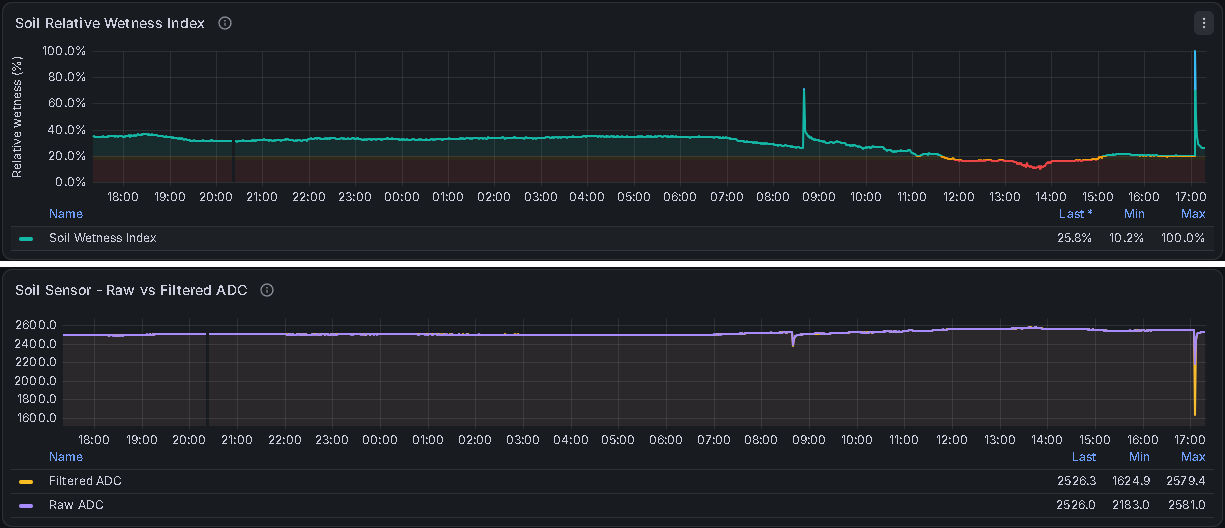
\includegraphics[width=\columnwidth]{grafana-watering.png}
\caption{Wetness index and ADC traces on 5 November. The two peaks occur near the reported watering times of 08:30 and 17:00.}
\label{fig:watering}
\end{topicfigure}

\subsection{CSV Completeness and Data Gaps}
The Grafana Explore file saved on 3 November 2026 covers displayed timestamps from 29 October at 09:54 through 3 November at 17:00. A CSV parser counted 5,860 data rows after the header and found 5,860 distinct timestamp, device, and plant keys. All rows have the three soil fields. Of these, 5,844 have all five thermal fields and 16 lack all thermal fields. Thus 99.7\% of exported rows contain both measurement families. A pivoted table row can combine multiple fields and measurements at one minute. Raw InfluxDB points and scheduled archive rows must be counted separately. The Explore CSV has no data-source tag column.

\begin{table}[!t]
\caption{Recounted Grafana Explore rows by displayed date. The first and last dates are partial.}
\label{tab:daily}
\centering\footnotesize
\begin{tabular}{@{}lrrr@{}}
\hline
Date in 2026 & Rows & With soil & With thermal\\ \hline
29 Oct. & 823 & 823 & 823\\
30 Oct. & 1369 & 1369 & 1369\\
31 Oct. & 1340 & 1340 & 1340\\
1 Nov. & 872 & 872 & 872\\
2 Nov. & 1396 & 1396 & 1380\\
3 Nov. & 60 & 60 & 60\\ \hline
Total & 5860 & 5860 & 5844\\ \hline
\end{tabular}
\end{table}

Comparing adjacent timestamps found 141 separations longer than one minute. The largest were 967 minutes (2 November at 23:52 to 3 November at 15:59), 581 minutes (31 October at 23:05 to 1 November at 08:46), and 34 minutes (30 October at 13:05 to 13:39). Across the inclusive export span, 5,860 of 7,627 nominal minute slots appear (76.8\%). The 1,767 absent slots describe this file's coverage. Device downtime, Wi-Fi or TLS failure, ingestion failure, or export query behavior could each produce missing rows. Attribution requires correlated timestamps from firmware, ingest, and database logs.

The two-day view in Fig.~\ref{fig:two-days} shows a thermal gap around midday on 4 November while soil readings continue in the same interval. Red marks a gap that exceeds 180 seconds between received points. It does not identify the failed component. The two-day dashboard table shows 2,794 rows. That count applies to the dashboard selection and is separate from the earlier 5,860-row CSV audit.

\begin{topicfigure}
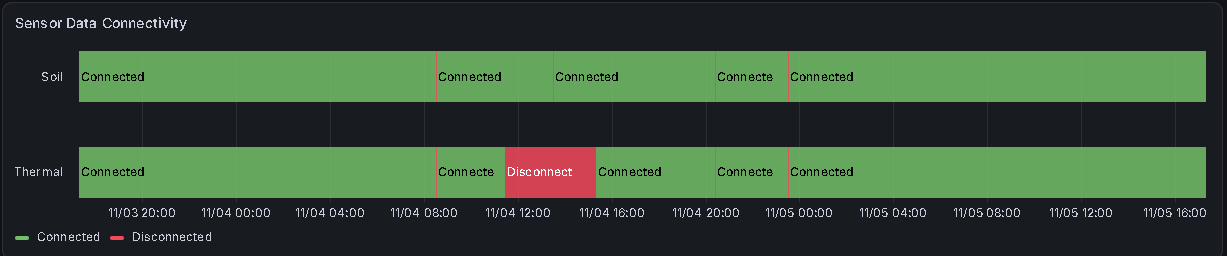
\includegraphics[width=\columnwidth]{grafana-two-days.png}
\caption{Two-day telemetry availability view. A red section appears in the thermal row around midday on 4 November, while the soil row stays green.}
\label{fig:two-days}
\end{topicfigure}

\subsection{Grafana Visualization and Status Thresholds}
Figure~\ref{fig:grafana-overview} shows the complete dashboard, including readings, status, trends, data gaps, the thermal matrix, and recent history.

\begin{figure*}[!t]
\centering
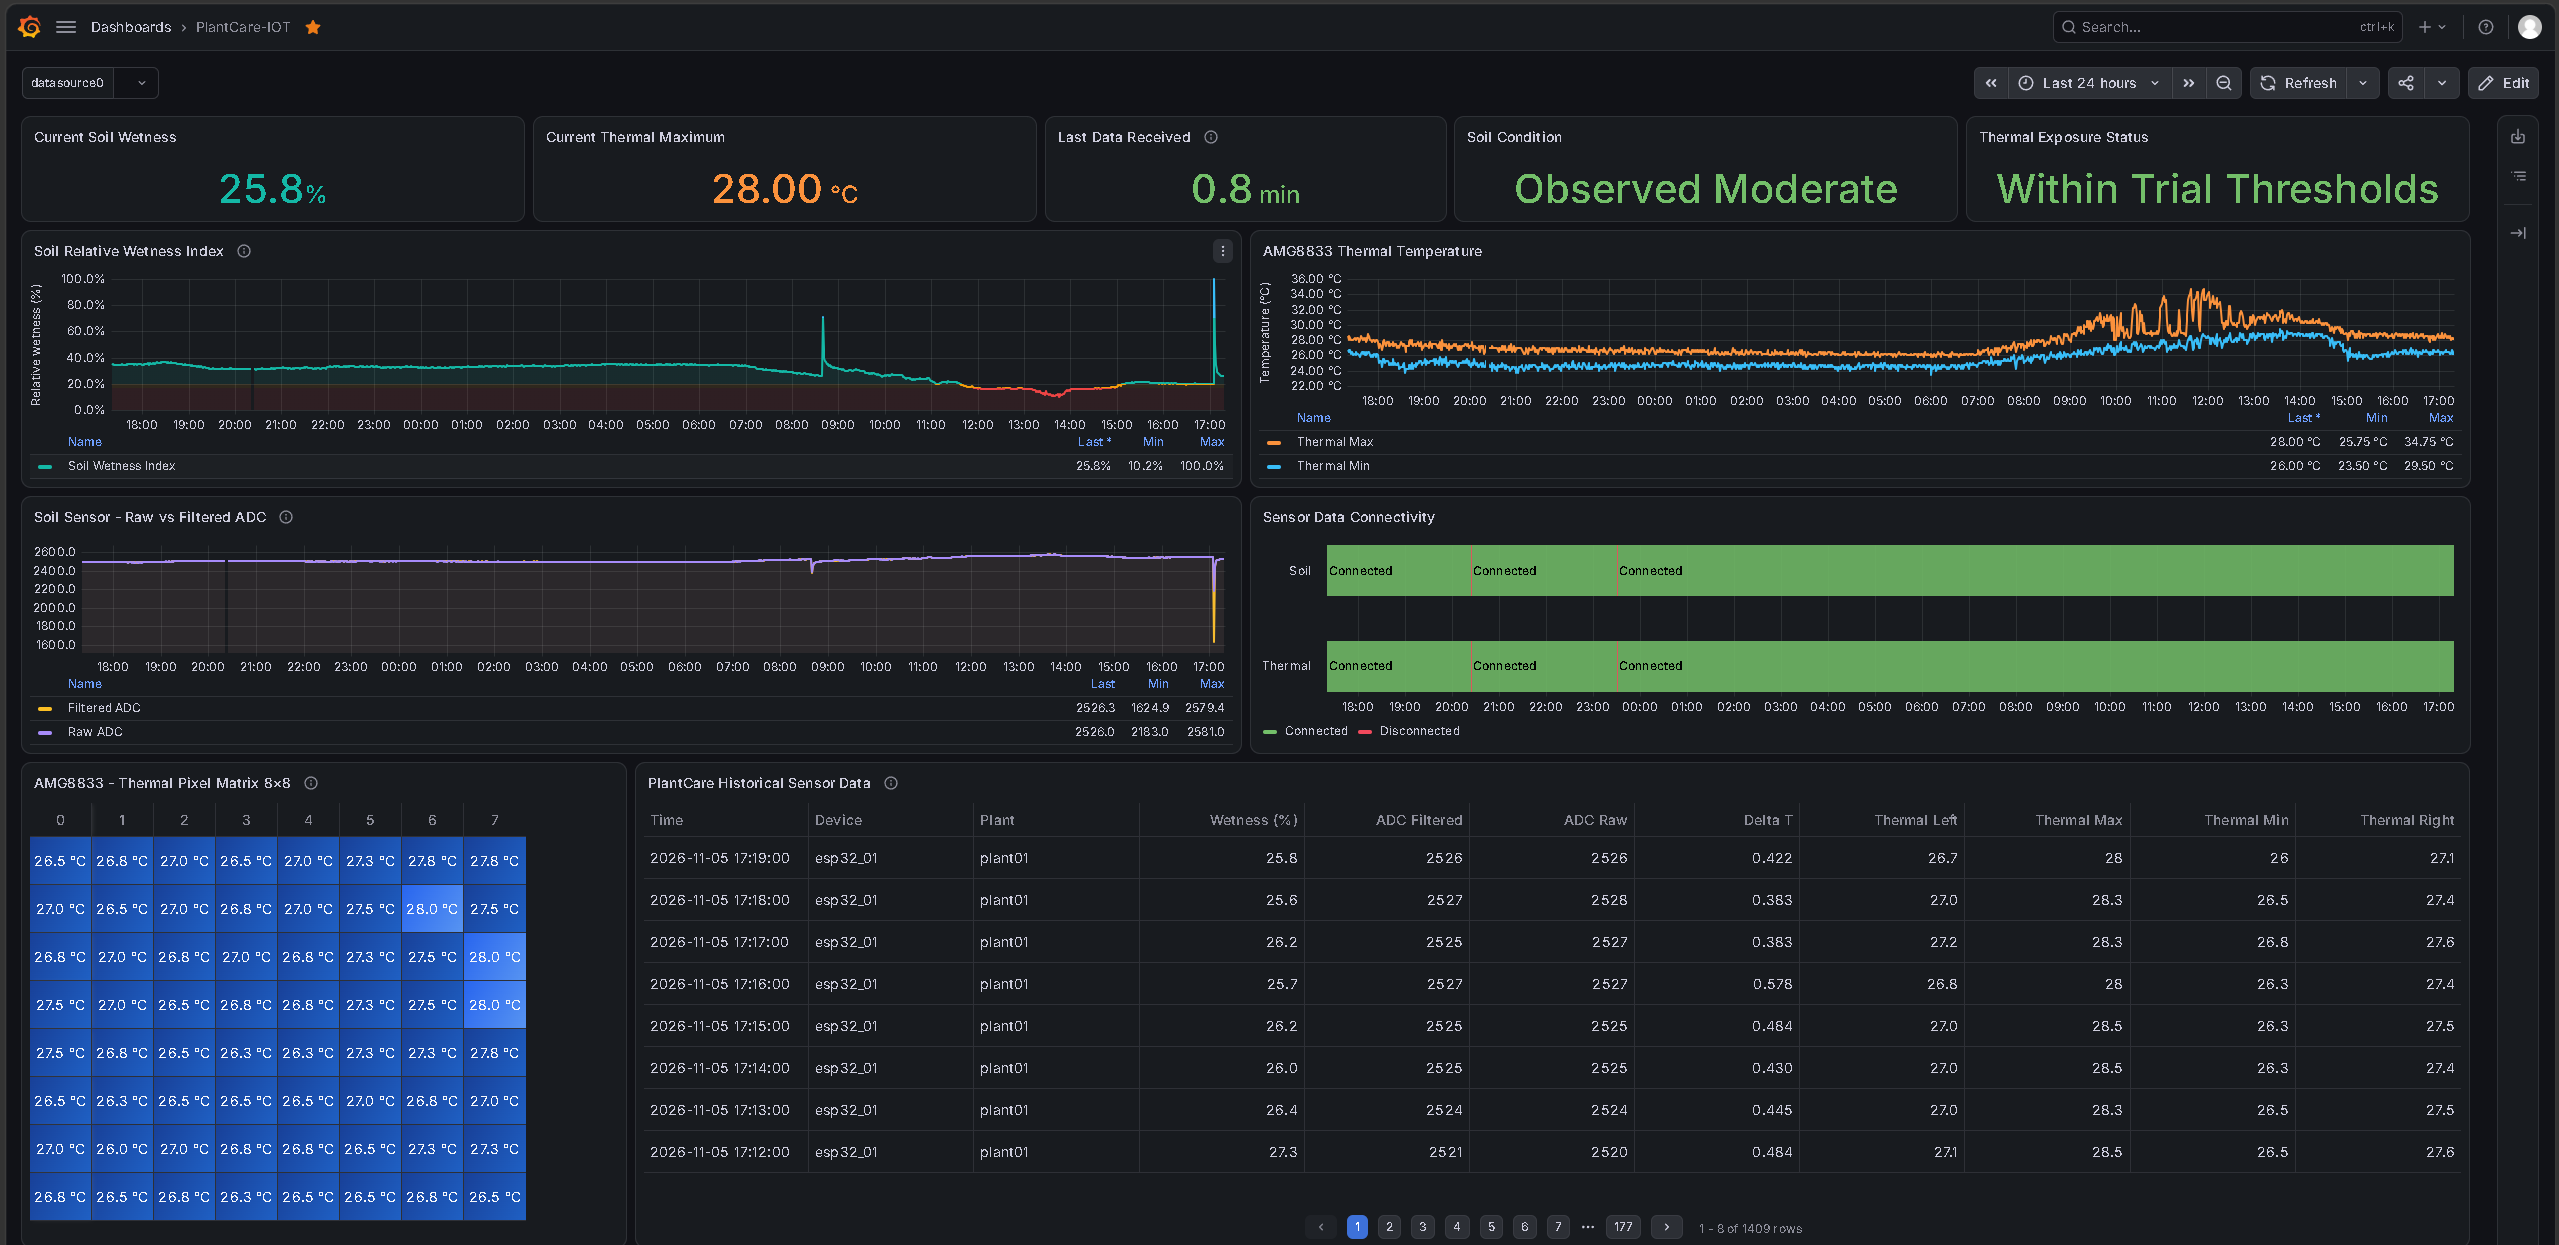
\includegraphics[width=.88\textwidth]{grafana-overview.png}
\caption{Full PlantCare Grafana dashboard in the 24-hour view on 5 November 2026. The bottom-left panel shows the 8$\times$8 thermal pixel matrix. Figs.~\ref{fig:watering} and~\ref{fig:two-days} show the watering and gap details.}
\label{fig:grafana-overview}
\end{figure*}

In the 24-hour capture, the latest soil index was 25.8\%, the thermal maximum was $28.00\degc$, and the most recent soil reading was about 0.8 min old. Grafana showed \emph{Observed Moderate} and \emph{Within Trial Thresholds}. These cards summarize the latest available readings using the trial rules.

\paragraph{Thermal pixel matrix}
The heatmap is a Grafana table with eight rows and eight columns. Flux reads the latest value for each pixel field in the selected time range and pivots the field names into grid positions. Each cell shows the measured temperature in Celsius and uses a fixed temperature color scale. This view shows warmer and cooler areas within the sensor's field of view, which can include the pot or nearby surfaces. The query selects the latest point for each field separately. It is a spatial view for one device, and the reading-age card still matters when checking freshness.

The soil bands at 17, 20, and 70\% reflect readings observed before and after watering. Grafana Stat value mappings render them as labels \cite{grafana}. The current maximum panel uses orange below $35\degc$ and red from $35\degc$. The exported numeric tiles query the previous 15 minutes. Both status cards use a three-minute window, and thermal status requires a recent pair at the same timestamp. Table~\ref{tab:thresholds} lists the saved rule boundaries, with the elevated maximum taking priority.

\begin{table}[!t]
\caption{Experimental dashboard rules. Wetness is a relative index. The thermal rules are evaluated top to bottom.}
\label{tab:thresholds}
\centering\footnotesize
\begin{tabular}{@{}L{.41\columnwidth}L{.53\columnwidth}@{}}
\hline
Reading & Trial label and color\\ \hline
$W<17\%$ & Observed Dry (red)\\
$17\%\leq W<20\%$ & Low Wetness (amber)\\
$20\%\leq W<70\%$ & Observed Moderate (teal)\\
$W\geq70\%$ & High Wetness Reading (blue)\\ \hline
$T_{\max}\geq35\degc$ & Elevated Temperature (red)\\
$\Delta T\geq2\degc$ with $T_{\max}<35\degc$ & Uneven Thermal Exposure (amber)\\
Both below thresholds & Within Trial Thresholds (green)\\
No recent complete input & No recent data\\ \hline
\end{tabular}
\end{table}

During panel editing, the generic InfluxDB source produced a bucket error. Both new captures show the status cards populated. The export includes a data-source selector, while the panel queries retain a fixed InfluxDB data-source identifier. A new deployment must rebind those queries to its own source. Its no-value text is \emph{No recent data}, and the saved status panels have a green base threshold. Interpret the text and freshness before relying on color. A bucket error and a successful query with no recent points require different diagnosis.

Offline application of the saved bands assigns 4,203 soil rows to Observed Dry, 35 to Low Wetness, 1,621 to Observed Moderate, and 1 to High Wetness Reading. The 5,844 complete thermal rows have a maximum-temperature range of $22.8$ to $34.5\degc$ and a recorded difference from $0$ to $1.31\degc$. They all fall below the thermal rule boundaries. Controlled tests are needed for the elevated and uneven thermal states. Validating plant-health interpretations would also require independent observations.

\subsection{Cloud-Only Baseline and Required Benchmarks}
Table~\ref{tab:bench} records the remaining course measurements. For the cloud-only control, replay the same sensor sequence through equivalent services on a cloud VM. Hold rate, payload, and protocol constant to isolate placement. Run a separate protocol comparison with the same payload on a normal link and a defined impaired link. Record the conditions and repetitions.

\begin{table}[!t]
\caption{Required quantitative evaluation and current evidence status.}
\label{tab:bench}
\centering\footnotesize
\begin{tabular}{@{}L{.35\columnwidth}L{.60\columnwidth}@{}}
\hline
Measurement & Method and status\\ \hline
Gateway and VM CPU/memory & \code{sysbench} CPU events/s and memory MiB/s. No paired host measurements.\\
Database disk I/O & \code{dd} read/write throughput on an isolated test volume (MiB/s). Unmeasured.\\
Link capacity and loss & \code{iperf3} TCP throughput and UDP loss/jitter under the same link profile \cite{iperf}. Unmeasured.\\
Latency & Report p50 and p95 in ms from a timestamped input to durable query visibility. Unmeasured.\\
Bandwidth savings & Capture HTTPS and MQTT bytes per delivered sample, including handshakes and retries. Unmeasured.\\
Power efficiency & Integrate measured supply power over a fixed trial and divide by delivered samples (J/sample). Unmeasured.\\ \hline
\end{tabular}
\end{table}

\code{iperf3} characterizes the link, and captures from the two application paths quantify protocol overhead. Record timestamps at source, acceptance, persistence, and query visibility. Compare bytes over equal-duration trials and report delivery completeness with any savings. The cloud-only comparison remains unmeasured.

\section{Conclusion and Future Work}
PlantCare lets the owner see what the two sensors are reading at the pot and review their history in Grafana. Soil ADC dropped after all four recorded watering trials. The Grafana views show two reported watering responses, a thermal gap, and the spatial pattern in the infrared frame. The ESP32 sends real readings over HTTPS, while the separate MQTT branch is for debugging. The project demonstrates monitoring for one pot. The available evidence does not establish water savings, plant stress, uptime, or energy efficiency.

A follow-up trial could repeat measured watering across several pots and compare the readings with an independent soil moisture measurement. Recording water volume, sensor placement, and event times would help explain differences between pots. A separate connection-loss test would show how quickly data resumes and which readings are lost.
